\documentclass[11pt]{article}

\usepackage[margin=1in]{geometry}
\usepackage{microtype}
\usepackage{booktabs}
\usepackage{tabularx}
\usepackage{array}
\usepackage{amsmath}
\usepackage{amssymb}
\usepackage{mathtools}
\usepackage{graphicx}
\usepackage{xcolor}
\usepackage{tikz}
\usetikzlibrary{arrows.meta,positioning,fit}
\usepackage[numbers,sort&compress]{natbib}
\usepackage[hidelinks]{hyperref}
\usepackage[nameinlink,noabbrev]{cleveref}

\newcommand{\rcqasyn}{RC-QASyn}
\newcommand{\draftstatus}[1]{\textcolor{gray}{\textsf{[#1]}}}
\newcommand{\papertodo}[2]{\textcolor{red!70!black}{\textsf{TODO[#1]: #2}}}

\title{Risk-Calibrated Quality-Aware Synthetic Dataset Construction}
\author{Anonymous Author(s)}
\date{PAPER v0.1 --- \today}

\begin{document}

\maketitle
\begin{abstract}
Synthetic records can be individually plausible while collectively forming a
poor dataset: accepted records may repeat one another, concentrate around a
small region of support, omit important subgroups, or fail to improve a
downstream task. We formulate \rcqasyn{} as a research direction that treats
synthetic-data creation as sequential dataset construction rather than
one-shot generation followed by a single filter. Its core separates
record-level validity from dataset-level quality, represents validator outputs
as scoped heterogeneous evidence, and proposes calibrated fusion for
risk-aware acceptance decisions. We describe a reproducible evaluation design
spanning deterministic rules, an uncalibrated language-model judge, copying
and support diagnostics, human record-validity annotation, intrinsic metrics,
and downstream utility. This provisional manuscript reports the implemented
experimental foundation and development observations; human annotation is in
progress, and calibration, risk-aware control, and final benchmark evaluation
remain pending. Localized repair and richer dataset optimization are possible
later extensions rather than experimentally validated components.
% TODO[RESULTS]: replace after final benchmark and completed human evaluation.
\end{abstract}


\section{Introduction}
\label{sec:introduction}

Synthetic data is increasingly used to supplement scarce observations, test
data-intensive workflows, support model development, and reduce dependence on
direct access to sensitive or restricted records. In tabular learning, the
design space now spans conditional adversarial generators
\citep{xu2019ctgan}, language-model generators
\citep{borisov2023great,solatorio2023realtabformer}, and diffusion-based
approaches \citep{kotelnikov2023tabddpm,zhang2024tabsyn}. Language models also
make class-conditioned generation and task-specific prompting readily
accessible, including in imbalanced-data settings \citep{kim2024epic}. These
capabilities make generation easier to deploy, but they do not by themselves
establish that the resulting collection is fit for scientific or predictive
use.

A plausible-looking row is only one part of a usable synthetic dataset. A
candidate can violate a schema, omit a required field, leave the observed
categorical domain, contradict its requested class, or be statistically or
semantically implausible. Even records that pass such checks may create a weak
dataset through exact or near redundancy, narrow support, distorted
class-conditional structure, or poor downstream utility. Some deployments add
privacy- and fairness-specific obligations that cannot be inferred from
realism alone; this draft treats corresponding evaluators as domain-dependent
extensions rather than part of the initial empirical core. Work on constrained
tabular generation shows why distributional fit and declared domain
constraints are distinct requirements
\citep{stoian2024realistic}, while multidimensional auditing separates
fidelity, diversity, and generalization rather than treating quality as a
single number \citep{alaa2022faithful}.
% TODO[CITATION]: add primary privacy and fairness evaluation sources before
% making claims about any particular protection or fairness criterion.

Existing generation and evaluation methods illuminate different parts of this
problem. Controlled generator benchmarks hold experimental factors fixed and
combine intrinsic and downstream views \citep{kim2025evaluating}; synthetic
data surveys likewise organize generation, curation, and evaluation as
separate stages \citep{long2024survey}. Other work develops distributional
metrics, constraint enforcement, or model-based critics. These strands are
complementary, but their outputs do not share a natural scale or scope. A
schema failure is a field- or record-level fact, a judge score is an uncertain
assessment, a duplicate count is a dataset property, and downstream utility is
an outcome of a learning pipeline. Treating these signals as interchangeable
can hide both missing evidence and disagreement.

This motivates a central distinction: record validity and dataset value are
related but not equivalent. An exact copy of a valid training example may be a
well-formed member of the target class, yet contribute no new support to an
accepted synthetic collection. Conversely, a novel candidate may improve
coverage while carrying a local defect that should not be accepted unchanged.
Evaluation therefore has to ask both whether a candidate is acceptable in
isolation and what changes when that candidate is added to the dataset. The
latter question is conditional on the evolving collection and cannot be
answered by a fixed per-record score.

We study \rcqasyn{} as a sequential dataset-construction framework. A
generator proposes a candidate under a dataset specification and a
TRAIN-derived context. Record- and dataset-level evaluators emit scoped
evidence; a future calibration and fusion stage preserves uncertainty and
provenance; and a risk-aware controller makes acceptance decisions without
reducing all evidence to an undifferentiated quality score. The current
repository implements the reproducible generation, paired-baseline,
diagnostic, and human-audit infrastructure needed to study this core. It does
not yet implement the proposed M2+ evaluator suite, calibration, evidence
fusion, or controller. Localized repair and richer dataset optimization are
later extensions whose inclusion in the final system depends on evidence from
the core experiments.

\paragraph{Research questions.}
RQ1 and RQ2 are the immediate questions for the human-audited development
study. RQ3 tests the core proposed decision method after M2 implementation;
RQ4 and RQ5 are longer-range questions that need not be answered by the first
complete paper.

\begin{description}
  \item[RQ1.] To what extent do structural rules, statistical-support
    evidence, and language-model critics identify human-judged defects in
    synthetic records?
  \item[RQ2.] How does record-level validity differ from dataset-level quality,
    including redundancy, support coverage, and distributional fidelity?
  \item[RQ3.] Can calibrated heterogeneous evidence provide more reliable
    acceptance decisions than raw generation, deterministic filtering, or one
    uncalibrated language-model judge? \emph{This core question requires M2+
    implementation and final evaluation.}
  \item[RQ4.] Can defect-localized repair improve accepted-data quality more
    efficiently than complete regeneration? \emph{This extension is not yet
    implemented.}
  \item[RQ5.] Can dataset-level marginal-contribution control improve
    diversity, coverage, and downstream utility without sacrificing record
    validity? \emph{This longer-range control question remains pending.}
\end{description}

\paragraph{Intended contributions and current status.}
The current work establishes a formulation that separates record-level
validity from dataset-level quality, a reproducible paired-baseline evaluation
framework, copying and support diagnostics, and a blinded human-ground-truth
protocol. We implement these elements and evaluate the diagnostics only in
development. We propose, but have not yet validated, calibrated heterogeneous
evidence fusion and a risk-aware decision controller. Localized repair and
sophisticated marginal-contribution optimization are secondary extensions.
Accordingly, ``Risk-Calibrated'' names the intended final method and research
hypothesis; the current implementation provides no calibrated risk guarantee.
Superiority, statistical significance, and final-benchmark claims remain
open.

\section{Related Work}
\label{sec:related-work}

\subsection{Synthetic Tabular Data Generation}

Tabular generators must jointly model heterogeneous variables, irregular
continuous distributions, imbalanced categories, and inter-column
dependencies. CTGAN addresses several of these difficulties through
mode-specific normalization, conditional sampling, and adversarial training
\citep{xu2019ctgan}. More recent diffusion approaches represent another model
family. TabDDPM adapts denoising diffusion to mixed numerical and categorical
features \citep{kotelnikov2023tabddpm}, while TabSyn applies score-based
diffusion in a learned latent space \citep{zhang2024tabsyn}. These methods
primarily concern how to learn and sample a data distribution; their existence
does not remove the need for independent dataset auditing.

Language-model approaches serialize rows and use autoregressive sequence
models to represent tabular distributions. GReaT demonstrates conditional
generation from arbitrary observed feature subsets
\citep{borisov2023great}. REaLTabFormer extends transformer-based generation
to both independent tables and parent--child relational settings, and includes
mechanisms intended to detect or reduce copying
\citep{solatorio2023realtabformer}. These approaches broaden the generator
class relevant to our problem, but \rcqasyn{} is generator-agnostic: its focus
is the evidence and control process around candidate records rather than a new
generative model.

\subsection{LLM-Based Synthetic Data and Augmentation}

LLM-driven synthetic-data research commonly separates prompting and
generation from curation and evaluation \citep{long2024survey}. For imbalanced
tabular classification, EPIC shows that class-balanced demonstrations,
grouping, and consistent formatting can materially affect generation
\citep{kim2024epic}. This is particularly relevant to class-conditioned
reference examples: demonstrations can convey useful structure, but they can
also anchor generation to a small visible subset. Our development protocol
therefore records reference identities and measures exact reference copying
separately from other TRAIN matches.

Generator evaluation is also sensitive to uncontrolled experimental choices.
AgoraBench fixes data, prompts, student models, and evaluation within a setting
when comparing language models as data generators, and considers several
intrinsic signals alongside downstream performance
\citep{kim2025evaluating}. We adopt the same broad principle of paired
comparison: B1, B2, and B3 operate on one persisted candidate pool. Our present
experiments concern small tabular development datasets rather than the text,
code, and reasoning settings studied by AgoraBench.

\subsection{Synthetic Data Quality Evaluation}

Synthetic-data quality is inherently plural. Marginal distribution distances
can reveal feature-wise shifts, association measures can expose relationship
distortion, and downstream tasks estimate whether a synthetic training set
supports prediction. None establishes the others. Alaa et al. formalize a
related separation through alpha-precision, beta-recall, and authenticity,
targeting fidelity, diversity, and generalization at both sample and
distribution levels \citep{alaa2022faithful}. Constraint-based work likewise
shows that distributional resemblance does not guarantee compliance with
domain knowledge \citep{stoian2024realistic}.

The current study uses transparent classical distances, correlation error,
redundancy measures, class-conditional views, and TRTR/TSTR utility. It does
not implement alpha-precision, beta-recall, or authenticity. Exact TRAIN
matching and nearest-neighbour support distances are reported as development
diagnostics, not as calibrated validity scores.
% TODO[CITATION]: verify primary sources for the final privacy, fairness, and
% subgroup-coverage evaluation protocol after those experiments are frozen.

\subsection{LLM-Based Critics and Self-Evaluation}

Language models can provide flexible rubric-based judgments where complete
deterministic rules are unavailable. Studies of LLM-as-a-judge evaluation,
however, document position, verbosity, self-enhancement, and reasoning biases
\citep{zheng2023judging}. Their results concern open-ended assistant responses
and do not establish reliability for tabular record validity. SelfCheckGPT
uses variation across sampled responses as a black-box factuality signal
\citep{manakul2023selfcheckgpt}; this is conceptually relevant to uncertainty
and disagreement, but sentence-level factual consistency is not equivalent to
schema, target-class, or support validity in a structured record.

These limitations motivate treating a critic output as one evidence item with
recorded provenance and uncertainty. The B3 critic in our implemented
development pipeline is intentionally a narrow baseline: one static threshold,
one judge, no calibration, no ensemble, and no evidence fusion. Moreover, the
generator and B3 judge use the same model, creating a plausible correlated
self-evaluation failure mode that the human audit is designed to examine.

\subsection{Uncertainty, Calibration, and Risk Control}

Calibration asks whether a model's reported confidence corresponds to its
empirical correctness frequency. Post-hoc methods such as temperature scaling
can improve calibration in conventional classification settings
\citep{guo2017calibration}. Risk-control methods address a different goal:
selecting a procedure or threshold so that a specified loss is controlled
under stated assumptions. Conformal risk control extends conformal ideas to
bounded monotone losses \citep{angelopoulos2022conformal}.

\rcqasyn{} draws conceptual guidance from these distinctions but does not
assume that an LLM's self-reported score is a calibrated probability. Nor does
it claim that existing conformal guarantees transfer directly to dependent,
heterogeneous validator evidence. Determining suitable calibration targets,
held-out data, risk functions, and dependence assumptions is part of M2+.

\subsection{Iterative Refinement and Repair}

Iterative language-model methods demonstrate that generation need not end
after a first draft. Self-Refine alternates model-generated feedback and
revision \citep{madaan2023selfrefine}; Chain-of-Verification separates draft,
verification questions, independent answers, and final revision for factual
generation \citep{dhuliawala2024chain}. These methods support the general idea
that critique can guide another action, but they do not by themselves provide
dependency-aware field repair for tabular records. A local edit may invalidate
related fields, and a repaired candidate must be revalidated under the same
specification. The proposed repair subsystem therefore remains a distinct,
optional extension rather than an assumed consequence of generic
self-refinement.

\subsection{Research Gap}

Prior work provides strong generators, multidimensional metrics, constraint
mechanisms, model-based critics, calibration methods, and iterative revision
strategies. We find limited integration of these strands into a sequential
tabular dataset-construction process that (i) preserves evidence scope and
provenance, (ii) separates record validity from dataset-level evidence, and
(iii) distinguishes evaluator uncertainty from acceptance risk before making
a decision. This gap is narrower than a claim that no prior system combines
validation and generation. It identifies the core open question addressed by
\rcqasyn{}: whether calibrated heterogeneous record and dataset evidence can
improve decisions under a reproducible, human-audited protocol. Repair and
richer dataset optimization are possible extensions of that core.

\section{Problem Formulation}
\label{sec:formulation}

\subsection{Sequential Synthetic Dataset Construction}

Let $D_{\mathrm{train}}=\{(z_j,y_j)\}_{j=1}^{n}$ denote the real TRAIN split,
where $z_j$ contains the non-target fields and $y_j$ is the target. Let $S$
denote the dataset specification: field names and types, the target definition,
categorical domains, missing-value policy, and any declared logical or domain
constraints. For a requested class or generation condition $c$, a generator
$G$ proposes a candidate record
\begin{equation}
  x_t \sim G\!\left(\,\cdot \mid S,c,C_{\mathrm{train}}\right),
  \label{eq:generation}
\end{equation}
where $C_{\mathrm{train}}$ is context derived only from $D_{\mathrm{train}}$.
The real TEST split is excluded from $C_{\mathrm{train}}$, validator fitting,
and controller design.

The accepted synthetic dataset evolves with the decision sequence. Writing
$D_{\mathrm{syn}}^{(t)}$ for the collection before evaluating $x_t$, an
acceptance produces
\begin{equation}
  D_{\mathrm{syn}}^{(t+1)}
  =D_{\mathrm{syn}}^{(t)}\cup\{x_t\},
  \label{eq:accepted-update}
\end{equation}
whereas rejection leaves the collection unchanged. Repair and regeneration
create a new candidate version or a new candidate, respectively, and therefore
require another validation pass. This sequential view matters because a
candidate's dataset-level value depends on records accepted earlier.

\subsection{Quality, Risk, Uncertainty, and Contribution}

We distinguish four objects. Record-level quality is a vector
\begin{equation}
  Q_R(x_t)=
  \bigl(q_{\mathrm{schema}},q_{\mathrm{constraint}},
        q_{\mathrm{logical}},q_{\mathrm{semantic}},q_{\mathrm{support}}\bigr),
  \label{eq:record-quality}
\end{equation}
whose components need not be commensurate. A binary validity decision, when a
protocol requires one, is a policy over relevant components rather than a
definition of quality itself.

Record-level risk $R_R(x_t)$ concerns the expected consequence of accepting a
candidate under a stated use and loss. The same defect can therefore carry
different risk in exploratory augmentation and a high-stakes deployment.
Evaluator uncertainty $U_R(x_t)$ describes confidence, disagreement, missing
evidence, or limited applicability of the evaluators. It is not a synonym for
risk: an evaluator may be certain about a low-consequence defect or uncertain
about a high-consequence one.

Finally, dataset marginal contribution is conditional on the current accepted
set:
\begin{equation}
  \Delta_D\!\left(x_t\mid D_{\mathrm{syn}}^{(t)}\right)
  =\bigl(\Delta_{\mathrm{novelty}},
         \Delta_{\mathrm{coverage}},
         \Delta_{\mathrm{fidelity}},
         \Delta_{\mathrm{utility}}\bigr).
  \label{eq:dataset-contribution}
\end{equation}
These components may trade off and are not collapsed into one weighted score
in this draft. Individual validity does not imply positive marginal
contribution across all dataset-quality dimensions. An exact copy can be
structurally and semantically valid while adding no new support. Conversely,
novelty cannot excuse an invalid record.

\subsection{Scoped Heterogeneous Evidence}

For candidate $x$, let
\begin{equation}
  \mathcal{E}(x)=\{e_1(x),\ldots,e_m(x)\}
  \label{eq:evidence-set}
\end{equation}
be a set of evidence items. Conceptually, each item is a tuple
\begin{equation}
  e_i=(s_i,d_i,v_i,u_i,p_i),
  \label{eq:evidence-item}
\end{equation}
where $s_i\in\{\mathsf{FIELD},\mathsf{RECORD},\mathsf{SUBGROUP},
\mathsf{DATASET}\}$ is scope; $d_i$ is a quality or risk dimension; $v_i$ is
a score, verdict, or structured finding; $u_i$ describes confidence or
uncertainty; and $p_i$ records provenance. Evidence at different scopes is not
automatically comparable. A failed type check can identify a field-level
violation, while a coverage statistic describes the accepted dataset and
cannot be attributed to one field in the same way.

The current repository contract implements versioned evidence identifiers,
quality dimension, verdict, severity, optional score and confidence, affected
fields, provenance, latency, cost, and creation time. A dedicated scope field
is part of the proposed architecture and is not yet implemented. This
difference is recorded because the mathematical object describes the intended
M2+ interface rather than overstating the M1 contract.

\subsection{Decision Problem}

The intended controller applies a policy
\begin{equation}
  a_t=\pi\!\left(\mathcal{E}(x_t),
                  D_{\mathrm{syn}}^{(t)},S,\rho\right),
  \quad
  a_t\in\{\mathsf{ACCEPT},\mathsf{REPAIR},
           \mathsf{REGENERATE},\mathsf{REJECT}\},
  \label{eq:controller}
\end{equation}
where $\rho$ denotes declared risk constraints and operating preferences.
Revalidation is an internal transition required after repair; the repository
action contract reserves it explicitly. Repair defines a longer-range
extension of the action space and is not required for the first core
acceptance-decision comparison. The policy should retain abstention or
unknown states when evidence is missing and should not treat an uncalibrated
critic score as a correctness probability. Equation~\eqref{eq:controller}
defines the proposed decision problem. No learned fusion or risk-constrained
controller is implemented in the present milestone.

\section{Proposed RC-QASyn Framework}
\label{sec:method}

\rcqasyn{} is an intended architecture for constructing a synthetic dataset
under explicit quality and risk requirements. Its core comprises scoped
record- and dataset-level evidence, calibration and fusion, and risk-aware
decision control around a replaceable generator. Localized repair,
privacy/fairness or domain-factual modules, and richer dataset optimization are
extensions that can be added when the core evidence justifies them. The
architecture is shown in \cref{fig:framework}; visual status distinguishes
implemented M1 infrastructure, M1.5 diagnostics, proposed core components, and
later extensions.

\begin{figure}[t]
  \centering
  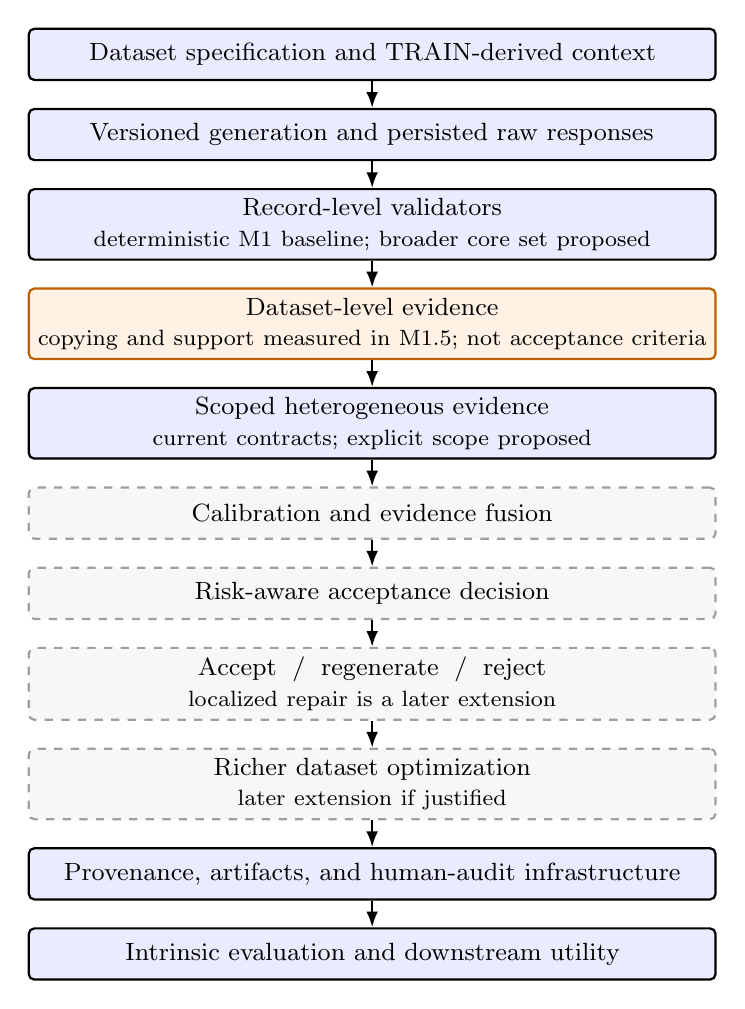
\begin{tikzpicture}[
    node distance=3.4mm,
    every node/.style={font=\small, align=center, minimum height=6.5mm,
      text width=0.70\linewidth, rounded corners=2pt},
    implemented/.style={draw=black, fill=blue!8, thick},
    diagnostic/.style={draw=orange!75!black, fill=orange!10, thick},
    proposed/.style={draw=gray!75, fill=gray!6, dashed, thick},
    flow/.style={-{Latex[length=2mm]}, thick}
  ]
    \node[implemented] (spec) {Dataset specification and TRAIN-derived context};
    \node[implemented, below=of spec] (gen) {Versioned generation and persisted raw responses};
    \node[implemented, below=of gen] (val) {Record-level validators\\\footnotesize deterministic M1 baseline; broader core set proposed};
    \node[diagnostic, below=of val] (diag) {Dataset-level evidence\\\footnotesize copying and support measured in M1.5; not acceptance criteria};
    \node[implemented, below=of diag] (evidence) {Scoped heterogeneous evidence\\\footnotesize current contracts; explicit scope proposed};
    \node[proposed, below=of evidence] (fusion) {Calibration and evidence fusion};
    \node[proposed, below=of fusion] (control) {Risk-aware acceptance decision};
    \node[proposed, below=of control] (action) {Accept \;/\; regenerate \;/\; reject\\\footnotesize localized repair is a later extension};
    \node[proposed, below=of action] (dataset) {Richer dataset optimization\\\footnotesize later extension if justified};
    \node[implemented, below=of dataset] (audit) {Provenance, artifacts, and human-audit infrastructure};
    \node[implemented, below=of audit] (utility) {Intrinsic evaluation and downstream utility};

    \draw[flow] (spec) -- (gen);
    \draw[flow] (gen) -- (val);
    \draw[flow] (val) -- (diag);
    \draw[flow] (diag) -- (evidence);
    \draw[flow] (evidence) -- (fusion);
    \draw[flow] (fusion) -- (control);
    \draw[flow] (control) -- (action);
    \draw[flow] (action) -- (dataset);
    \draw[flow] (dataset) -- (audit);
    \draw[flow] (audit) -- (utility);
  \end{tikzpicture}
  \caption{Intended \rcqasyn{} pipeline. Solid blue nodes denote implemented
  M1 infrastructure, orange denotes M1.5 diagnostic analysis, and dashed gray
  nodes denote unevaluated proposed components. The central proposed path is
  scoped evidence, calibration/fusion, and risk-aware decision making;
  localized repair and richer optimization are extensions.}
  \label{fig:framework}
\end{figure}


\subsection{Specification and Generation}

The specification makes the schema, target, categorical domains,
missing-value policy, class condition, generation objective, and provenance
requirements explicit. Generation uses only a TRAIN-derived profile and,
when enabled, deterministic class-aware TRAIN examples. Prompts and provider
settings are versioned. Raw responses are preserved before parsing, so a
transport or parse failure remains observable instead of being silently
repaired. This stage and its reproducibility machinery are implemented.

The generator is not assumed to certify its own output. A prompt may describe
observed ranges or request target consistency, but compliance is established
only by evidence produced after generation. This separation prevents prompt
instructions from being mistaken for enforced constraints.

\subsection{Independent Validators and Heterogeneous Evidence}

Each validator should answer a narrow question and emit a structured evidence
item rather than a final global judgment. Deterministic schema, domain,
missing-value, target-condition, observed-range, and duplicate checks exist in
the current baseline pipeline. The core proposed evaluator set adds
independent statistical-support and task-relevant logical or semantic
evidence. Factual verification, privacy, and fairness require domain- and
use-specific definitions and are treated as optional modules, not as
implemented or guaranteed capabilities in PAPER v0.1.

Validator independence is an experimental objective, not an assumption that
errors are statistically independent. Two evaluators may share training data,
model families, prompts, or representations and therefore make correlated
errors. Provenance and evaluator identity are retained so calibration and
ablation can measure such dependence rather than conceal it.

\subsection{Record-Level and Dataset-Level Evidence}
\label{sec:record-dataset-evidence}

Record-level evidence includes schema correctness, required-field presence,
categorical validity, target consistency, local statistical support, and
logical or semantic plausibility. It supports statements about one candidate
or one of its fields. Dataset-level evidence instead includes exact and near
redundancy, prompt-reference copying, support and class-conditional coverage,
distributional fidelity, subgroup representation, and downstream utility.

The distinction changes how evidence is acted upon. A target mismatch is a
candidate defect; adding many copies of a correct minority example is a
collection-level failure. A record can therefore satisfy record-level validity
while contributing little new support to the dataset. \rcqasyn{} proposes to
retain both views and to prevent a dataset-level redundancy finding from being
misreported as record invalidity.

\subsection{Calibration and Evidence Fusion}

The proposed calibration layer maps evaluator outputs to empirically supported
reliability statements on held-out, human-labelled development data. Fusion
then combines evidence without erasing scope, missingness, or provenance. A
field-level hard violation may dominate an acceptance decision, while
uncertain semantic evidence may call for review or regeneration. Dataset-level
coverage evidence should influence selection among otherwise acceptable
records rather than retroactively redefine their structural validity.

This draft deliberately does not specify a universal weighted sum. Calibration
targets, dependence handling, fusion rules, and risk guarantees must be frozen
and evaluated after the human audit. The current B3 score is uncalibrated and
is not an implementation of this layer.

\subsection{Risk-Aware Decision Control}

Given calibrated evidence and declared risk constraints, the intended
controller selects whether a candidate should be accepted, regenerated, or
rejected under a frozen loss and operating policy. The action contract also
reserves repair, but the core empirical question is whether calibrated scoped
evidence yields more reliable acceptance decisions than the paired baselines.
No action-selection policy or calibrated risk guarantee is implemented in the
present milestone.

\subsection{Dataset Evidence and Audit}

Dataset-level evidence evaluates marginal redundancy, coverage, fidelity, and
prospective utility relative to $D_{\mathrm{syn}}^{(t)}$. Keeping this evidence
separate from record validity is part of the core formulation. A future
controller may use it to defer or decline a valid but redundant record, but
thresholds and objectives must be derived without access to REAL TEST labels
or statistics.

M1.5 implements diagnostic measurements of exact copying and TRAIN-support
distance, but these measurements do not yet control acceptance. The audit
layer is already partly implemented: run manifests, resolved configuration,
prompt and seed plans, provider traces, candidates, decisions, evidence,
metrics, copying/support diagnostics, and blinded human-review identities are
persisted for analysis.

\subsection{Later-Stage Extensions}

Localized repair could be useful when a defect and its dependency set can be
identified and revalidated; complete regeneration remains the comparison when
localization is unsafe or uneconomical. Richer dataset optimization could
select among valid candidates using multiple marginal-contribution objectives.
Neither mechanism is necessary to test the core record/dataset evidence and
calibrated-decision hypothesis. No repair operator or dataset optimizer is
currently implemented, and neither is presented as an established advantage.

\subsection{Implementation Status Summary}

\begin{table}[t]
  \centering
  \caption{Framework status in PAPER v0.1. ``Development'' denotes pilot
  diagnostics, not final benchmark validation.}
  \label{tab:framework-status}
  \begin{tabularx}{\linewidth}{@{}lXl@{}}
    \toprule
    Component & Current repository support & Research status \\
    \midrule
    Specification and generation & Versioned configs/prompts, TRAIN-only
      context, persisted raw responses and provenance & Core---implemented \\
    Baseline validators & Deterministic B2 checks and one B3 critic over a
      shared candidate pool & Core---implemented \\
    Copying/support analysis & Exact-copy categories and TRAIN-distance
      summaries without acceptance thresholds & Core---development \\
    Human audit & Blinded export/import, overlap, agreement, and adjudication
      infrastructure; labels incomplete & Core---results pending \\
    Explicit evidence scope & FIELD/RECORD/SUBGROUP/DATASET interface & Core---proposed \\
    Calibration and fusion & Reliability estimation and heterogeneous fusion & Core---proposed \\
    Risk-aware controller & Evidence-based acceptance policy & Core---proposed \\
    Localized repair & Dependency-aware edit and revalidation & Extension \\
    Richer dataset optimization & Multi-objective marginal-contribution
      selection & Extension \\
    \bottomrule
  \end{tabularx}
\end{table}

\section{Experimental Methodology}
\label{sec:experiments}

This section describes the implemented M1--M1.6 development protocol. It is
intended to make the pilot auditable and to freeze the comparison design before
the proposed \rcqasyn{} components are evaluated. The three datasets are
development datasets, not the complete final benchmark.

\subsection{Datasets, Registry, and Splits}

Dataset definitions are versioned in \texttt{configs/datasets/}. Source and
acquisition records live under \texttt{data/manifests/}, while each run persists the
resolved TRAIN profile and split manifest in its \texttt{dataset/} directory. The
current development set covers moderate, severe, and extreme binary class
imbalance and includes one mixed-type dataset. Exact characteristics and the
committed splits appear in \cref{tab:development-datasets}.

\begin{table}[t]
  \centering
  \caption{Development datasets and committed deterministic stratified splits.
  Class counts are full-dataset negative/positive counts; IR is
  majority/minority. These are pilot datasets, not the complete final
  benchmark.}
  \label{tab:development-datasets}
  \small
  \begin{tabularx}{\linewidth}{@{}lrrrrrX@{}}
    \toprule
    Dataset & Rows & Num. & Cat. & Neg./Pos. & IR & TRAIN / TEST \\
    \midrule
    page-blocks0 & 5,472 & 10 & 0 & 4,913 / 559 & 8.79 & 4,377 / 1,095 \\
    Ecoli4       &   336 &  7 & 0 &   316 / 20  & 15.80 & 269 / 67 \\
    Abalone19    & 4,174 &  7 & 1 & 4,142 / 32  & 129.44 & 3,340 / 834 \\
    \bottomrule
  \end{tabularx}
\end{table}


Each dataset is split once by deterministic stratified sampling under root
seed 42. Profiles, observed numeric summaries, categorical domains, class
proportions, and reference examples are computed from TRAIN only. REAL TEST is
reserved for downstream evaluation: it is not used in prompt construction,
deterministic validation, judge prompts, model fitting, or threshold design.
The run manifests record \texttt{no\_test\_leakage=true}. The current final-benchmark
plan is broader but remains unevaluated, as summarized in
\cref{tab:planned-benchmark}.

\begin{table}[t]
  \centering
  \caption{Planned final-benchmark roles. Inclusion and protocol remain to be
  frozen; listing a dataset does not imply that a final experiment exists.}
  \label{tab:planned-benchmark}
  \small
  \begin{tabularx}{\linewidth}{@{}lXl@{}}
    \toprule
    Dataset & Intended stress-test role & Status \\
    \midrule
    Default Credit Card & Mild imbalance / control & Planned \\
    HTRU2 & Moderate real-world imbalance & Planned \\
    Ecoli4 & Small-data scarcity & Development only \\
    Musk & High dimensionality & Planned \\
    Mammography & Severe imbalance & Planned \\
    Bank Marketing & Mixed numerical/categorical features & Planned \\
    Abalone19 & Extreme imbalance & Development only \\
    \bottomrule
  \end{tabularx}
  \par\smallskip
  \footnotesize APS and Satimage-2 remain optional candidates in the research
  plan; neither is claimed as part of a frozen benchmark.
\end{table}


\subsection{P1 Generation Protocol}
\label{sec:p1-protocol}

P1 uses the local OpenAI-compatible Ollama endpoint convention
\texttt{http://127.0.0.1:11434/v1}; this deployment choice is not a scientific
contribution. The generator is \texttt{gemma4:e4b}. For each dataset, the configuration
requests 200 records in explicit class-conditioned batches: 100 negative and
100 positive, with batch size five. The TRAIN context contains a compact
profile and four deterministic reference records, two per class. Generation
uses prompt version v2, temperature 0.7, a 2,048-token output limit, and a
120-second timeout.

Prompt v2 requests one JSON object with a single \texttt{records} array. This
transport wrapper was introduced to match the provider's JSON-object response
format; it is separate from the feature schema and does not enforce field
validity. Raw provider output is stored before parsing. Parse errors, wrong
outer shapes, and item-level failures are retained rather than clipped,
imputed, or silently regenerated.

The root seed and configured provider base seed are both 42. A cryptographic
derivation based on SHA-256 maps
\begin{equation}
  (\text{root seed},\text{dataset},\text{requested class},\text{batch index},
  \text{base seed})
  \longmapsto \text{provider seed},
  \label{eq:seed-derivation}
\end{equation}
with the result reduced to the provider's unsigned 32-bit range. The complete
seed plan is computed before generation and checked for collisions across all
scheduled dataset/class/batch tuples. Provider traces bind every candidate to
the corresponding batch index and derived seed.

\subsection{Paired Baselines}
\label{sec:baselines}

All three baselines operate on the same persisted parseable candidate pool.
They differ only in the acceptance policy.

\paragraph{B1---raw generation.}
B1 accepts every parseable candidate. It performs no filtering, repair, or
regeneration; parse failures remain outside the candidate pool and are
reported separately.

\paragraph{B2---deterministic filtering.}
B2 runs five independent checks: exact declared schema and primitive numeric
types; TRAIN-observed categorical domains; the declared missing-value policy;
agreement between the generated target and requested class; and observed TRAIN
numeric ranges. Schema, invalid-domain, rejected-missing, and target-condition
failures have HIGH severity. Observed-range findings have MEDIUM severity and
are warnings by default. The configured policy rejects HIGH and CRITICAL
evidence. In addition, B2 rejects every repeated canonical candidate after its
first occurrence. It does not learn a fusion rule and does not modify records.

\paragraph{B3---single LLM judge.}
B3 makes one judge call per parseable candidate using \texttt{gemma4:e4b}, the same
model used for generation. The judge runs at temperature 0 with prompt version
v1, strict JSON-object parsing, a static threshold of 0.7, and rejection of
malformed outputs. A candidate is accepted only when the parsed verdict is
PASS or WARN and its score reaches the threshold. The score is self-reported
and uncalibrated; B3 uses no ensemble, evidence fusion, external factual
verification, repair, or adaptive threshold. Sharing the generator model
creates a possible correlated-error and self-evaluation limitation rather than
a benefit.

\subsection{Intrinsic and Downstream Metrics}

Numeric features are compared between REAL TRAIN and accepted synthetic data
with the two-sample Kolmogorov--Smirnov statistic and one-dimensional
Wasserstein distance. Categorical features, including the target, use total
variation distance and Jensen--Shannon divergence. Pearson and Spearman
dependence error is the mean absolute difference between corresponding
off-diagonal correlations over numerical feature pairs.

Diversity outputs include the number of unique canonical rows, exact duplicate
count and rate, base-two categorical entropy, numerical variance relative to
REAL TRAIN, and the number of unique categorical combinations. Numeric,
categorical, and duplicate views are also reported by target class. Empty and
degenerate cases carry explicit statuses and null values rather than synthetic
zeros.

Downstream utility uses train-real/test-real (TRTR) as a reference and
train-synthetic/test-real (TSTR) as the synthetic-data condition. The
implemented classifiers are logistic regression with standardized numerical
features and a \texttt{liblinear} solver, and a 50-tree random forest; categorical
features are imputed and one-hot encoded. Metrics are F1, average precision
(reported under both \texttt{average\_precision} and \texttt{pr\_auc}), Matthews correlation
coefficient, balanced accuracy, and AUROC. No single metric is sufficient:
distributional similarity does not imply useful decision boundaries,
downstream utility does not reveal redundancy or constraint failures, and
record validity does not establish dataset coverage.

\subsection{Copying and Support Diagnostics}
\label{sec:diagnostics}

M1.5 computes three independent exact-copy indicators for every raw candidate:
whether it repeats an earlier synthetic record, equals a TRAIN reference shown
in its prompt, or equals a TRAIN record not shown in the prompt. These
categories distinguish generation-scale redundancy from visible-example
anchoring and contact with unshown TRAIN data. Exact TRAIN matching is a
copying diagnostic; it is not called privacy leakage in this study.

Support diagnostics measure Euclidean nearest-neighbour distance to REAL TRAIN
after numerical z-score standardization with TRAIN mean and population
standard deviation. Zero-variance numeric columns are removed. Categorical
features are one-hot encoded over TRAIN domains with unit weight. The reports
include nearest TRAIN, nearest same-class TRAIN, and nearest other-class TRAIN
distance where defined. These distances are representation-dependent,
learning-free diagnostics with no validity threshold, probability
interpretation, or effect on B1/B2/B3 decisions.

\subsection{Blinded Human Evaluation}
\label{sec:human-evaluation}

The master audit contains 120 unique-prioritized records, 40 from each
development dataset. Its manifest records overlapping selection-stratum hits:
18 accepted by all three baselines, eight B2/B3 disagreements, seven B2
rejections, one B3 rejection, 18 high-distance and 16 low-distance records, 15
majority and 15 minority records, 15 non-copies, and seven reference copies.
Because these are overlapping priority hits, they are not intended to sum to
120.

Reviewer A receives all 120 records. Reviewer B receives a deterministic
40-record overlap selected with seed 42: 14 Abalone19, 14 Ecoli4, and 12
page-blocks0 records, balanced as 20 negative and 20 positive requested
classes. Reviewers see only an anonymous annotation ID, record ID, dataset,
requested class, serialized candidate, and the five human-entry fields. They
do not see B2/B3 decisions, B3 scores or reasons, copying flags, support
distances, provider metadata, or automated verdicts.

For blinded annotation, a human-valid record conforms to known schema and
domain semantics and is a plausible member of the requested class,
independently of redundancy within the synthetic dataset. Redundancy alone
does not make a record invalid. Reviewers assign a boolean validity label and
one or more controlled record-level failure types; severity, affected fields,
and \texttt{human\_notes} are optional. Agreement will be summarized with raw
agreement and Cohen's kappa on explicitly labelled overlap. Disagreements are
manually adjudicated and are never resolved automatically. Human annotation is
in progress, so no human-validity result appears in this draft.

\subsection{Reproducibility and Development Confounds}
\label{sec:reproducibility}

P1 was executed with Python 3.12.11. Each run stores resolved configuration,
dataset and split fingerprints, TRAIN profile, prompt hash and version,
generation plan, seed plan, provider traces, raw candidates, baseline
decisions/evidence, metrics, and diagnostics. The three P1 manifests identify
source commit \texttt{ab492bf294b563e4b165755692ac8edb8f3dd2be} but also record
\texttt{git\_dirty=true}; the persisted artifacts, not a claim of a clean historical
checkout, are therefore the primary record of the runs.

An earlier P0-v2 protocol reused one provider seed across same-class batches.
The provider replayed raw batches, creating an artificial 75\% exact duplicate
rate on each development dataset. The problem was diagnosed as a seed
confound, and the per-dataset/class/batch derivation in
\cref{eq:seed-derivation} was implemented with a pre-run uniqueness guard.
P0-v3 and P1 use the corrected protocol. Confounded P0-v2 diversity values are
not evidence about generator quality.

One further artifact discrepancy remains open: the Ecoli4 P1 run contains 201
parseable records although the configuration requested 200. The extra record
came from the persisted generation output and is not silently discarded in
the reports. Consequently, Ecoli4 rates in this draft use the recorded pool
denominator where stated, and the count anomaly is treated as a development
limitation requiring resolution before the final benchmark.

\section{Results}
\label{sec:results}

\subsection{Development and Pilot Observations}
\label{sec:pilot-results}

This subsection reports descriptive P1 development diagnostics. It is not a
final benchmark, contains one run per dataset, and supports no statistical
significance or generator-ranking claim. The corrected JSON-object transport
produced persisted parseable pools at or above the requested size: 200 records
for Abalone19, 201 for Ecoli4, and 200 for page-blocks0. The extra Ecoli4 record
is the unresolved over-generation anomaly described in
\cref{sec:reproducibility}; rates below use the recorded pool denominator.

\begin{table}[t]
  \centering
  \caption{P1 development diagnostics. Percentages use each persisted
  parseable pool as denominator. ``Unshown'' means an exact match to a TRAIN
  row not used as a prompt reference. Disagreement is B2-reject/B3-accept.}
  \label{tab:p1-pilot-diagnostics}
  \resizebox{\linewidth}{!}{%
  \begin{tabular}{@{}lrrrrrrr@{}}
    \toprule
    Dataset & Pool & Duplicate (\%) & Reference (\%) & Unshown (\%) &
      B2 accept (\%) & B3 accept (\%) & Disagree ($n$) \\
    \midrule
    Abalone19    & 200 & 28.50 & 24.50 & 0.00 & 69.00 & 100.00 & 62 \\
    Ecoli4       & 201 & 10.45 & 10.95 & 0.00 & 86.57 &  99.50 & 26 \\
    page-blocks0 & 200 &  9.50 &  1.00 & 0.00 & 87.50 & 100.00 & 25 \\
    \bottomrule
  \end{tabular}}
\end{table}


Exact duplicate rates were 28.5\% for Abalone19, 10.45\% for Ecoli4, and
9.5\% for page-blocks0. Exact prompt-reference matches accounted for 24.5\%,
10.95\%, and 1.0\% of the same pools, respectively. No dataset contained an
exact match to a TRAIN record that had not been shown as a prompt reference.
The distinction matters: these results describe exact copying categories, not
semantic similarity or near copying.

The P0-v3 to P1 scaling comparison increased the configured request from 40 to
200 records per dataset under the corrected seed protocol. Duplicate rates
rose from 17.5\% to 28.5\% for Abalone19, from 5.0\% to 10.45\% for Ecoli4,
and from 7.5\% to 9.5\% for page-blocks0. With one run at each scale, these are
descriptive observations only. They motivate repeated-seed and repeated-split
experiments; they do not estimate a scaling law.

B2 accepted 138/200 Abalone19, 174/201 Ecoli4, and 175/200 page-blocks0
records. B3 accepted every Abalone19 and page-blocks0 record and 200/201
Ecoli4 records. Thus, the current same-model, record-wise B3 baseline exhibited
little discrimination in P1; this observation does not establish that
language-model judges are generally ineffective. The disagreement report
contains 62, 26, and 25 cases where B2 rejected and B3 accepted. Of these, 57,
21, and 19 were classified as
dataset-redundancy cases, while 5, 5, and 6 were structural/domain cases. The
counts show that the policies operationalize different concepts; human labels
are required before interpreting either policy as the better record-validity
critic.

TRAIN-support summaries were successfully produced for each pool using the
representation in \cref{sec:diagnostics}. Their raw distances are not compared
across datasets because scale after feature construction, dimensionality, and
class support differ. No support threshold was selected, and support distance
did not alter an acceptance decision.

The repository also contains pilot TRTR/TSTR outputs. PAPER v0.1 does not use
them as comparative evidence: the evaluation has one split per dataset, the
minority test sets are very small, and several logistic-regression TSTR entries
are undefined in the committed reports. These artifacts remain part of the
evidence record and require protocol review before final utility claims.

\subsection{Human Ground-Truth Audit}
\label{sec:human-results}

The blinded sample contains 120 records and the committed manifest confirms
that all human-entry columns were blank when the sample was generated.
Annotation is in progress.

% TODO[HUMAN]: insert reviewer completion counts, confusion analyses, raw
% agreement, Cohen's kappa, adjudication outcomes, and uncertainty intervals.
\papertodo{HUMAN}{Results require completed blinded annotation and adjudication.}

\subsection{Final Benchmark}
\label{sec:final-benchmark-results}

No final benchmark has been run. Dataset inclusion, repeated-split design,
uncertainty intervals, and statistical tests must be frozen before this
subsection is populated.

% TODO[RESULTS]: replace all planned table cells only from versioned final
% benchmark artifacts.
\papertodo{RESULTS}{Final benchmark and statistical analysis are pending.}

\subsection{Ablations}
\label{sec:results-ablations}

No proposed M2+ component is implemented, so no ablation outcome is available.
The planned factorial questions are specified in \cref{sec:ablations}; detailed
future-only table shells are retained in the non-rendered manuscript notes.

\begin{table}[t]
  \centering
  \caption{Pending human critic benchmark. All entries require completed
  annotation and adjudication.}
  \label{tab:future-human-benchmark}
  \begin{tabular}{@{}lrrrr@{}}
    \toprule
    Critic & Precision & Recall & F1 & Agreement \\
    \midrule
    B2 deterministic & -- & -- & -- & -- \\
    B3 single judge & -- & -- & -- & -- \\
    Proposed fused evidence & -- & -- & -- & -- \\
    \bottomrule
  \end{tabular}
\end{table}

\begin{table}[t]
  \centering
  \caption{Planned final B1/B2/B3/\rcqasyn{} comparison; \rcqasyn{} is not
  implemented.}
  \label{tab:future-baselines}
  \begin{tabular}{@{}lrrrr@{}}
    \toprule
    System & Human validity & Coverage & TSTR & Cost \\
    \midrule
    B1 raw & -- & -- & -- & -- \\
    B2 deterministic & -- & -- & -- & -- \\
    B3 single judge & -- & -- & -- & -- \\
    Proposed \rcqasyn{} & -- & -- & -- & -- \\
    \bottomrule
  \end{tabular}
\end{table}


\section{Discussion}
\label{sec:discussion}

This section separates observations supported by the development runs from
hypotheses that require human labels, M2 implementation, and repeated final
evaluation.

\subsection{Development Observations}

\paragraph{Syntax is a necessary but weak success criterion.}

The transport correction demonstrates a basic methodological point: reliable
structured output is necessary before scientific evaluation is meaningful.
Once the JSON boundary is stable, however, parseability says little about
schema compliance, target consistency, plausibility, redundancy, coverage, or
utility. Future comparisons should therefore report transport and parse
failures separately from quality findings rather than rewarding a generator
for syntax alone.

\paragraph{Record validity and dataset quality lead to different decisions.}

The pilot B2/B3 disagreements are partly explained by policy rather than by
critic accuracy. B2 rejects repeated canonical candidates; the blinded human
task explicitly does not mark an otherwise sound record invalid merely because
it is redundant. A record-validity benchmark must therefore remove
duplicate-only B2 rejections from the structural-validity view, while a dataset
construction benchmark should retain them as evidence of low marginal value.
This separation is central to \rcqasyn{} and will be tested directly after
human annotation.

\paragraph{Self-judging and example anchoring.}

B3's near-universal acceptance in P1 cannot yet be interpreted as either
correct tolerance or critic failure. The judge and generator share a model,
and the human labels required to distinguish these explanations are pending.
The reference-copying diagnostics raise a parallel concern: class-aware
examples may improve conditioning while anchoring the generator to a small
visible support set. The magnitude varies across the three pilot datasets,
which argues for reporting reference identity and copying rather than treating
in-context examples as an unexamined implementation detail.

\paragraph{Scale and redundancy.}

Duplicates increased between P0-v3 and the larger P1 request for all three
development datasets. With one run at each scale, the study cannot establish a
trend or explain its cause.

\subsection{Hypotheses for Later Stages}

No implemented signal answers every evaluation question. Deterministic rules
are precise within their declared domain but do not establish semantic
plausibility; a language-model critic is flexible but potentially correlated
and uncalibrated; copying and support diagnostics describe dataset contact but
do not define record validity; downstream utility aggregates many upstream
effects. We therefore hypothesize that scoped heterogeneous evidence will be
more informative than any single critic and that calibration will improve
decision reliability. We separately hypothesize that dataset-aware control can
improve coverage and that localized repair can reduce action cost. None of
these hypotheses is established by P1; the latter two may remain extensions if
they are unnecessary for the core result.

% TODO[DISCUSSION]: revisit every interpretive claim after human adjudication,
% repeated splits, final benchmarks, and M2+ ablations.

\section{Ablation Study}
\label{sec:ablations}

All ablations in this section are planned. Their purpose is to freeze the
questions that a final implementation may need to answer, not to imply an
available outcome. The core sequence is record/dataset evidence, calibration,
fusion, and decision control; repair and richer optimization are extension
experiments. Detailed placeholder tables are preserved in
\texttt{notes/future\_experiment\_tables.tex} and are not rendered in this
professor draft.

\paragraph{Record-level validators.}
Starting from the complete record-level suite, remove structural rules,
statistical-support evidence, and semantic criticism one family at a time.
Measure human-invalid acceptance, human-valid rejection, failure-type recall,
and cost on the same candidate identities.

\paragraph{Dataset-level evaluators.}
Remove exact/near redundancy, support coverage, class-conditional coverage,
and subgroup control separately. Evaluate duplicate accumulation, coverage,
distributional fidelity, and downstream utility at matched accepted-set size.

\paragraph{Calibration and fusion.}
Compare raw B3 scores, separately calibrated evaluator outputs, and the frozen
heterogeneous fusion rule. Calibration data must be disjoint from final
evaluation records. Report reliability and selective-risk views rather than
accuracy alone.

\paragraph{Repair policy (extension).}
For candidates with a localizable defect, compare rejection, complete
regeneration, and localized repair followed by dependency-aware revalidation.
Measure human validity after action, residual defects, success per provider
call, tokens, latency, and cost.

\paragraph{Dataset construction (later-stage control).}
Compare acceptance without contribution control to redundancy-only, coverage-
only, and combined marginal-contribution policies. Repeat generation seeds and
real-data splits so that uncertainty is not conflated with one extreme-
imbalance partition.

% TODO[ABLATION]: populate only after M2+ interfaces and the final protocol are
% frozen and versioned.

\section{Limitations}
\label{sec:limitations}

The present evidence comes from three development datasets, one corrected P1
run per dataset, and one real TRAIN/TEST split per dataset. These datasets do
not span the intended final benchmark, and 200 requested records per dataset
provide limited evidence about scaling. Repeated generation seeds, repeated
real-data splits, uncertainty intervals, and predeclared statistical
comparisons are pending.

Human evaluation is incomplete and modest in size: Reviewer A receives 120
records and Reviewer B overlaps on 40. Even after adjudication, specialist
domain validity may be difficult for general annotators to judge, particularly
when feature names encode scientific measurements without sufficient domain
context. The final paper must report reviewer qualifications and any domain
guidance without exposing personal information.

Generation and B3 judging use the same local model. Their errors may therefore
be correlated, and findings may not generalize to other local models, hosted
models, prompts, decoding configurations, or model scales. B3's score is
uncalibrated. The proposed calibration, evidence fusion, and risk controller
have not been implemented or tested, so the current system provides no
calibrated risk control. Repair and richer dataset optimization are
unimplemented extensions.

Extreme imbalance makes single-split utility unstable. Ecoli4 and Abalone19
have only four and six positive records, respectively, in the committed TEST
splits. Several logistic-regression TSTR outputs are undefined, and the Ecoli4
generation pool contains 201 records despite a request for 200. Final utility
claims require correction or explicit accommodation of these issues.

Copying and nearest-neighbour support are diagnostics, not privacy measures.
Support distance depends on standardization, categorical encoding, feature
weighting, and dimensionality; it has no calibrated threshold in the current
study. Privacy and fairness validators, near-copy analysis, and subgroup-risk
evaluation are not implemented. Exact absence of a match to an unshown TRAIN
record must not be read as a privacy guarantee.

The historical P1 manifests record a dirty working tree, although they retain
resolved configuration, commit identity, prompts, traces, and outputs. The
implementation workbook could not be inspected with the required read-only
spreadsheet runtime during manuscript initialization and is not used as
evidence. Finally, the literature review is substantial but incomplete;
several repository notes remain unverified placeholders and are deliberately
excluded from the bibliography.

\section{Conclusion}
\label{sec:conclusion}

This work establishes a formulation, reproducible paired-baseline framework,
development diagnostic suite, and blinded human-grounded evaluation protocol
for studying quality-aware synthetic dataset construction. The formulation
separates record-level quality, acceptance risk, evaluator uncertainty, and a
candidate's marginal contribution to the evolving dataset.

The repository currently provides the reproducible generation and baseline
pipeline, corrected deterministic provider seeds, copying/support diagnostics,
and blinded human-audit infrastructure needed to test the proposed core. It
does not yet establish that \rcqasyn{} improves synthetic data or that
calibrated fusion and risk-aware control improve acceptance decisions. The
next scientific step is to complete and adjudicate the human audit, then use
those labels to freeze M2 evaluator and calibration designs. Repair and richer
optimization remain optional extensions. A final conclusion must wait for
that evidence, the implemented core components, repeated evaluation, and a
broader benchmark.

\section{Declarations and Author Contributions}
\label{sec:declarations}

\paragraph{Data and code availability.}
The development code, configurations, prompts, compact reports, run manifests,
and non-sensitive blinded review materials are maintained in the anonymous
project repository. Raw source datasets remain subject to their original
distribution terms. Large future artifacts will be transferred outside Git
with tracked SHA-256 manifests.

\paragraph{Ethics and human annotation.}
The current audit concerns synthetic tabular records and uses stable reviewer
identifiers rather than personal metadata. Reviewer comments belong only in
the intended human-notes field. Privacy and fairness evaluation is not yet
implemented, and no privacy guarantee is claimed.

\paragraph{Conflicts of interest.}
\papertodo{DECLARATION}{Authors to provide the final conflict-of-interest statement.}

\paragraph{Funding.}
\papertodo{DECLARATION}{Authors to provide funding and resource acknowledgements.}

\paragraph{Author contributions.}
\papertodo{CREDIT}{Replace anonymity-preserving placeholders with the final CRediT roles after author review.}


\bibliographystyle{plainnat}
\bibliography{references}

\end{document}
